\documentclass[11pt,a4paper]{article}
\usepackage[utf8x]{inputenc}
\usepackage{ucs}
\usepackage{graphicx}
\newcommand{\myc}[1]{\multicolumn{1}{c}{#1}}
\begin{document}
\begin{figure}
\begin{center}

\begin{tabular}{llll}

\includegraphics[scale=0.9]{surf1.eps} & 

\includegraphics[scale=0.9]{surf2.eps} & 

\includegraphics[scale=0.9]{surf3.eps} & 

\includegraphics[scale=0.9]{surf4.eps} \\
\rule[0mm]{0mm}{2mm} \\

\includegraphics[scale=0.9]{cont1.eps} & 
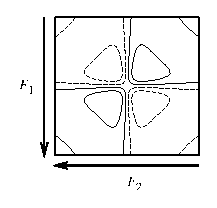
\includegraphics[scale=0.9]{cont2.eps} & 
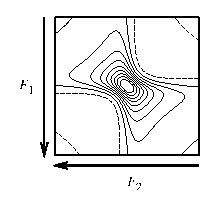
\includegraphics[scale=0.9]{cont3.eps} & 
\includegraphics[scale=0.9]{cont4.eps} \\
\myc{\raisebox{-0.5ex}[0pt]{Double}} &
\myc{\raisebox{-0.5ex}[0pt]{Double}} &
\myc{\raisebox{-0.5ex}[0pt]{Phase}} \\
\myc{Absorption} & 
\myc{Dispersion} & 
\myc{Twist} & 
\myc{\raisebox{1.25ex}[0pt]{Magnitude}}

\end{tabular}
\caption{Formes de raies en RMN 2D}
\end{center}
\end{figure}

\end{document}